\documentclass[letterpaper]{article}

%% Language and font encodings
\usepackage[english]{babel}
\usepackage[utf8x]{inputenc}
\usepackage[T1]{fontenc}

%% Sets page size and margins
\usepackage[letterpaper,top=3cm,bottom=2cm,left=2cm,right=2cm,marginparwidth=1.75cm]{geometry}

%% Useful packages
\usepackage{amsmath}
\usepackage{graphicx}
\usepackage[colorinlistoftodos]{todonotes}
\usepackage[colorlinks=true, allcolors=blue]{hyperref}
\usepackage{listings}

\usepackage[numbered,framed]{matlab-prettifier}
\let\ph\mlplaceholder % shorter macro
\lstMakeShortInline"

\lstset{
  style              = Matlab-editor,
  basicstyle         = \mlttfamily,
  escapechar         = ",
  mlshowsectionrules = true,
}

\title{EE576 HW 5}
\author{Jordan Caudill and Matt Ruffner}

\begin{document}
\maketitle

%%%%%%%%%%%%%%%%%%%%%%%%%%%%%%%%%%%%%%%%%%%%%%%%%%%%%%%%%%%%%%%%%%
%%%%%%%%%%%%%%%%%%%%%%%%%%%%%%%%%%%%%%%%%%%%%%%%%%%%%%%%%%%%%%%%%%
%%%%%%%%%%%%%%%%%%%%%%%%%%%%%%%%%%%%%%%%%%%%%%%%%%%%%%%%%%%%%%%%%%
\section{}
The difference between IoT blockchain and bitcoin blockchain is that:
\begin{enumerate}
    \item 
    The bitcoin blockchain prioritizes anonymity, while the IoT prioritizes identity. This is so you can use things like smart contracts to make transactions with authorized devices.
    \item 
    The IoT uses the PoS (Proof of Stake) and bitcoin uses PoW (Proof of Work). This is because the scale of associated with IoT devices would be too large to have it checked by everyone.
\end{enumerate}

\section{}

\subsection{}
The private key is used to create the signature (along with the public key). The signature is used to verif
 that the bitcoin transaction is taking place between the appropiate parties. The private key is kept secret, but is used to mathematically derive the public key. The public key is the address, which is how the bitcoin is known where to be sent.
\\
\\
The differences between the testnet transactions and the actual bitcoin transactions are the following:
\\
\begin{itemize}
    \item Default Bitcoin network protocol listen port is 18333 (instead of 8333)
    \item
Default RPC connection port is 18332 (instead of 8332)
\item
Bootstrapping uses different DNS seeds.
\item
A different value of ADDRESSVERSION field ensures no testnet Bitcoin addresses will work on the production network. (0x6F rather than 0x00)
\item
The protocol message header bytes are 0x0B110907 (instead of 0xF9BEB4D9)
\item
Minimum difficulty of 1.0 on testnet is equal to difficulty of 0.5 on mainnet. This means that the mainnet-equivalent of any testnet difficulty is half the testnet difficulty. In addition, if no block has been found in 20 minutes, the difficulty automatically resets back to the minimum for a single block, after which it returns to its previous value.
\item
A new genesis block
\item
The IsStandard() check is disabled so that non-standard transactions can be experimented with.
\end{itemize}
 (Source: https://en.bitcoin.it/wiki/Testnet)
\subsection{}
Write down the transaction hash and the faucet address as you will need it for the next step. How much bitcoin did you get and what was the tx fee?

\subsection{}
output of split script:
\begin{verbatim}
201 Created
{
  "tx": {
    "block_height": -1,
    "block_index": -1,
    "hash": "3cf4fd235c3d5d6d02e6431c19acae21a578a322a704a9f4a1f85c85e399b40f",
    "addresses": [
      "n3qmL3GcTF9rvbf6kqpuzLYQZCjrTSqaGk"
    ],
    "total": 50048336,
    "fees": 100000,
    "size": 430,
    "preference": "high",
    "relayed_by": "128.163.237.198",
    "received": "2019-02-25T01:30:55.793951859Z",
    "ver": 1,
    "double_spend": false,
    "vin_sz": 1,
    "vout_sz": 8,
    "confirmations": 0,
    "inputs": [
      {
        "prev_hash": "65e262e41987ed7652847afeb56ff975060abe9a89cf53330c6664a045dbedd9",
        "output_index": 1,
        "script": "483045022100e9817716cc0051e7acd6b2280c64c5410a542727e99f862028afcba19488aece02200ae7ae7ed1649455255182f9c53d440f6c954351908556cee9a980ff3e267c190121028bb1604765225d96539f6c0eccdc8ebed4f955e7951585f0101a27d9ccba8a80",
        "output_value": 50148336,
        "sequence": 4294967295,
        "addresses": [
          "n3qmL3GcTF9rvbf6kqpuzLYQZCjrTSqaGk"
        ],
        "script_type": "pay-to-pubkey-hash",
        "age": 1481390
      }
    ],
    "outputs": [
      {
        "value": 6256042,
        "script": "76a914f4e1844a7d5b631fa93d07861061029e0381ee6588ac",
        "addresses": [
          "n3qmL3GcTF9rvbf6kqpuzLYQZCjrTSqaGk"
        ],
        "script_type": "pay-to-pubkey-hash"
      },
      {
        "value": 6256042,
        "script": "76a914f4e1844a7d5b631fa93d07861061029e0381ee6588ac",
        "addresses": [
          "n3qmL3GcTF9rvbf6kqpuzLYQZCjrTSqaGk"
        ],
        "script_type": "pay-to-pubkey-hash"
      },
      {
        "value": 6256042,
        "script": "76a914f4e1844a7d5b631fa93d07861061029e0381ee6588ac",
        "addresses": [
          "n3qmL3GcTF9rvbf6kqpuzLYQZCjrTSqaGk"
        ],
        "script_type": "pay-to-pubkey-hash"
      },
      {
        "value": 6256042,
        "script": "76a914f4e1844a7d5b631fa93d07861061029e0381ee6588ac",
        "addresses": [
          "n3qmL3GcTF9rvbf6kqpuzLYQZCjrTSqaGk"
        ],
        "script_type": "pay-to-pubkey-hash"
      },
      {
        "value": 6256042,
        "script": "76a914f4e1844a7d5b631fa93d07861061029e0381ee6588ac",
        "addresses": [
          "n3qmL3GcTF9rvbf6kqpuzLYQZCjrTSqaGk"
        ],
        "script_type": "pay-to-pubkey-hash"
      },
      {
        "value": 6256042,
        "script": "76a914f4e1844a7d5b631fa93d07861061029e0381ee6588ac",
        "addresses": [
          "n3qmL3GcTF9rvbf6kqpuzLYQZCjrTSqaGk"
        ],
        "script_type": "pay-to-pubkey-hash"
      },
      {
        "value": 6256042,
        "script": "76a914f4e1844a7d5b631fa93d07861061029e0381ee6588ac",
        "addresses": [
          "n3qmL3GcTF9rvbf6kqpuzLYQZCjrTSqaGk"
        ],
        "script_type": "pay-to-pubkey-hash"
      },
      {
        "value": 6256042,
        "script": "76a914f4e1844a7d5b631fa93d07861061029e0381ee6588ac",
        "addresses": [
          "n3qmL3GcTF9rvbf6kqpuzLYQZCjrTSqaGk"
        ],
        "script_type": "pay-to-pubkey-hash"
      }
    ]
  }
}
\end{verbatim}

Shown in Fig. \ref{fig:split} is the proof of the split transaction, looked up on the blockcypher website by the transaction


\section{}
\texttt{split\_test\_coins.py} works in the following way:
\\
The code first creates the second half of the output signature that is based on the unhashed public key. The code then calculates the input transaction id (previous transaction) which contains the amount to spend and the amount needed). The code then creates the first half of the output signature using a hashed . After that it creates the output transaction. This is where the code splits it into n different outputs. This is done by dividing the amount to send by n and then using the second half of the signature to get the transaction. The code then calculates the transaction id. The code then hashes the signature, and the concatenates it to the end of the hashed private key. The code then verifies that everything matches and broadcast the results.
\\
\\


\section{}

\section{}


\begin{figure}[h!]
\centering
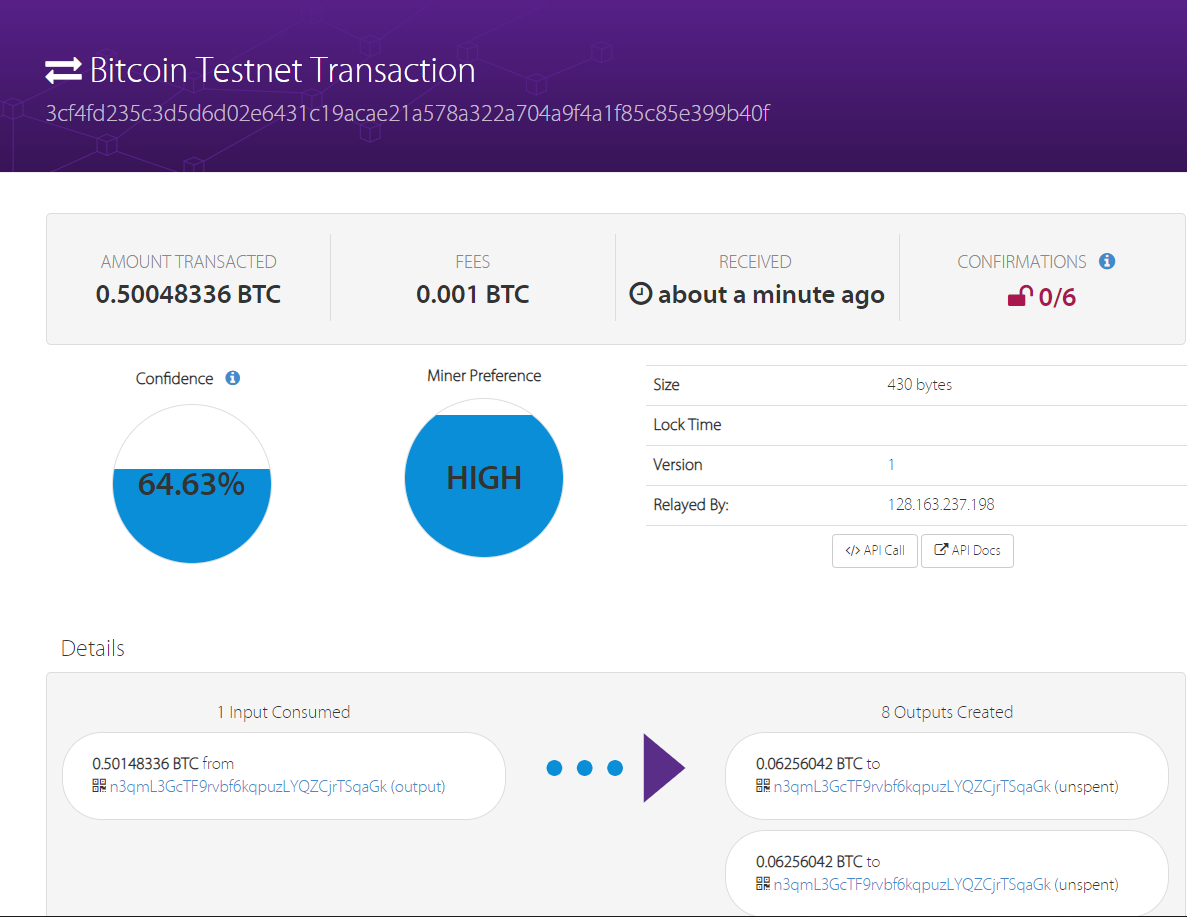
\includegraphics[width=\textwidth]{splitProof}
\caption{Proof of the splitting operation.}
\label{fig:split}
\end{figure}


\section{}

\begin{verbatim}
    $ python ex1.py
201 Created
{
  "tx": {
    "block_height": -1,
    "block_index": -1,
    "hash": "9552ebe79c21e3ce4eeaf07b1e0a65c781a91b744e3144dd9b85dbc857e1139c",
    "addresses": [
      "n3qmL3GcTF9rvbf6kqpuzLYQZCjrTSqaGk"
    ],
    "total": 6000000,
    "fees": 256042,
    "size": 191,
    "preference": "high",
    "relayed_by": "128.163.236.240",
    "received": "2019-02-28T23:12:51.718704911Z",
    "ver": 1,
    "double_spend": false,
    "vin_sz": 1,
    "vout_sz": 1,
    "confirmations": 0,
    "inputs": [
      {
        "prev_hash": "3cf4fd235c3d5d6d02e6431c19acae21a578a322a704a9f4a1f85c85e3                             99b40f",
        "output_index": 0,
        "script": "47304402205f75d5ea174427dd0888e315b99b0b80519e655d0f11766aafe                             02314c2a8131e02200e1651fa103bddd8be15b4f87ba0e52911cfe343da3d5eb017bc698bd7e3c72                             a0121028bb1604765225d96539f6c0eccdc8ebed4f955e7951585f0101a27d9ccba8a80",
        "output_value": 6256042,
        "sequence": 4294967295,
        "addresses": [
          "n3qmL3GcTF9rvbf6kqpuzLYQZCjrTSqaGk"
        ],
        "script_type": "pay-to-pubkey-hash",
        "age": 1481395
      }
    ],
    "outputs": [
      {
        "value": 6000000,
        "script": "76a914f4e1844a7d5b631fa93d07861061029e0381ee6588ac",
        "addresses": [
          "n3qmL3GcTF9rvbf6kqpuzLYQZCjrTSqaGk"
        ],
        "script_type": "pay-to-pubkey-hash"
      }
    ]
  }
}

\end{verbatim}


\section{}
\begin{verbatim}
from sys import exit
from bitcoin.core.script import *

from utils import *
from config import my_private_key, my_public_key, my_address, faucet_address
from ex1 import P2PKH_scriptPubKey
from ex2a import ex2a_txout_scriptPubKey


######################################################################
# TODO: set these parameters correctly
amount_to_send = 0.003
txid_to_spend = '5e02fff3f09250a4ab64a73517013c22d996045d604a8fbffd26a2948080e296'
utxo_index = 10
######################################################################

txin_scriptPubKey = ex2a_txout_scriptPubKey
######################################################################
# TODO: implement the scriptSig for redeeming the transaction created
# in  Exercise 2a.
#txin_scriptSig = [ 2534, -1444]
#txin_scriptSig = [ 2534, 1444 ]
#txin_scriptSig = [ b'\x09\xE6', b'\x05\xA4']
txin_scriptSig = [1444, 2534]
######################################################################
txout_scriptPubKey = P2PKH_scriptPubKey(faucet_address)

response = send_from_custom_transaction(
    amount_to_send, txid_to_spend, utxo_index,
    txin_scriptPubKey, txin_scriptSig, txout_scriptPubKey)
print(response.status_code, response.reason)
print(response.text)

\end{verbatim}



\section{}
\begin{verbatim}
from sys import exit
from bitcoin.core.script import *

from utils import *
from config import my_private_key, my_public_key, my_address, faucet_address
from ex1 import send_from_P2PKH_transaction


######################################################################
# TODO: Complete the scriptPubKey implementation for Exercise 2
#ex2a_txout_scriptPubKey = [ OP_EQUAL, OP_EQUALVERIFY ] 
ex2a_txout_scriptPubKey = [ OP_2DUP, OP_ADD, 3978, OP_EQUALVERIFY, OP_SUB, 1090, OP_EQUALVERIFY ] 
#ex2a_txout_scriptPubKey = [ OP_2DUP, OP_ADD, 3978, OP_EQUALVERIFY, OP_SUB, 1090, OP_EQUALVERIFY ] 
# [OP_DUP, OP_HASH160, faucet_address, OP_EQUALVERIFY, OP_CHECKSIG]
#[OP_ADD 2534 -1444]
######################################################################

if __name__ == '__main__':
    ######################################################################
    # TODO: set these parameters correctly
    amount_to_send = .0003
    txid_to_spend = (
        '5e02fff3f09250a4ab64a73517013c22d996045d604a8fbffd26a2948080e296')
    utxo_index = 10
    ######################################################################

    response = send_from_P2PKH_transaction(
        amount_to_send, txid_to_spend, utxo_index,
        ex2a_txout_scriptPubKey)
    print(response.status_code, response.reason)
    print(response.text)
\end{verbatim}
%%%%%%%%%%%%%%%%%%%%%%%%%%%%%%%%%%%%%%%%%%%%%%%%%%%%%%%%%%%%%%%%%%
%%%%%%%%%%%%%%%%%%%%%%%%%%%%%%%%%%%%%%%%%%%%%%%%%%%%%%%%%%%%%%%%%%
%%%%%%%%%%%%%%%%%%%%%%%%%%%%%%%%%%%%%%%%%%%%%%%%%%%%%%%%%%%%%%%%%%
\bibliographystyle{ieeetr}
\bibliography{refs.bib}

\end{document}